\chapter{The Best Model and Its Physics Reach}
\label{ch:best_model}

Chapters~5 through~8 established the architectural design choices for the
transformer classifier through a sequence of controlled ablations: physics-informed
input representations (Chapter~5), attention mechanism and bias interaction
(Chapter~6), model scaling and efficiency (Chapter~7), and global surrogate
optimisation (Chapter~8). This chapter synthesises those findings by evaluating the
best-performing model — Message-Interaction Attention (MIA) — against the physics
baseline on the primary four-top-quark classification task. Section~\ref{sec:ch9_selection}
identifies the best model and quantifies its AUROC improvement over the baseline.
Section~\ref{sec:ch9_discriminant} analyses the signal efficiency at physically
motivated background-rejection working points. Section~\ref{sec:ch9_physics_reach}
translates the classifier gain into an illustrative significance estimate under
HL-LHC conditions. Section~\ref{sec:ch9_summary} summarises the findings and
describes what a production physics analysis would require beyond this work.

% ─────────────────────────────────────────────────────────────────────────────
\section{Model Selection}
\label{sec:ch9_selection}

The MIA architecture (group \texttt{exp\_20260511-113827\_mia\_od\_followup\_seeds})
is the natural endpoint of the design exploration conducted in Chapters~5–8.
It combines differential attention (\wandbaxis{A3}\,$=$\,\texttt{differential}),
no attention-internal normalisation (\wandbaxis{A4}\,$=$\,\texttt{none}),
a Lorentz-scalar bias applied in split mode
(\wandbaxis{B1}\,$=$\,\texttt{lorentz\_scalar}, \wandbaxis{A3-a}\,$=$\,\texttt{split}),
and the scale and depth recommended by the Chapter~7 Pareto analysis. Each of these
choices was supported by the ablation evidence from the corresponding chapter; MIA
accumulates all recommended settings simultaneously.

The model was trained over five independent random seeds to obtain a stable estimate
of the test performance and its seed-to-seed variance. For comparison, the physics
baseline (group \texttt{exp\_20260306-190512\_4tbg\_physics\_baseline}, nine seeds)
implements the simplest viable transformer configuration: raw input features,
standard multi-head self-attention, no Lorentz-scalar bias, and the smallest
architecture preset. An additional reference point is provided by the Optuna
best trial (\num{150} Bayesian optimisation trials, AUROC\,$=$\,\num{0.8485}),
which confirms that MIA is not substantially outperformed by an unconstrained
hyperparameter search.

\Cref{tab:ch9_auroc_comparison} reports the test AUROC for all three models.
MIA achieves a mean AUROC of $\num{0.8504} \pm \num{0.0005}$ across five seeds,
compared with $\num{0.8063} \pm \num{0.0013}$ for the physics baseline — an absolute
improvement of $\Delta\,\mathrm{AUROC} \approx \num{0.044}$. The MIA seed spread
($\sigma = \num{0.0005}$) is narrower than that of the baseline ($\sigma = \num{0.0013}$),
indicating that the architectural improvements also stabilise training.

\begin{table}[h]
\centering\small
\begin{tabular}{llrr}
\toprule
Model & Group & Seeds & AUROC (mean\,$\pm$\,std) \\
\midrule
MIA (best model)     & \texttt{mia\_od\_followup\_seeds}   & 5 & $\num{0.8504} \pm \num{0.0005}$ \\
Optuna best trial    & \texttt{ch8\_optuna}                & 1 & \num{0.8485} (reference only) \\
Physics baseline     & \texttt{4tbg\_physics\_baseline}    & 9 & $\num{0.8063} \pm \num{0.0013}$ \\
\bottomrule
\end{tabular}
\caption{Test AUROC comparison for MIA, the Optuna best trial, and the physics baseline.
  The Optuna entry is a single best-trial result; no seed spread is available.
  All evaluations use the task 4t vs.\ ttH+ttW+ttWW+ttZ.}
\label{tab:ch9_auroc_comparison}
\end{table}

\Cref{fig:ch9_roc} shows the full ROC curves for MIA and the physics baseline.
The MIA mean curve (shaded band: one standard deviation across five seeds) lies
uniformly above the baseline curve across the entire false-positive-rate range,
with the separation widest in the high-background-rejection region. Vertical dotted
lines mark the three working points analysed in \cref{sec:ch9_discriminant}:
$1/B = 50$, $1/B = 100$, and $1/B = 1000$.

\begin{figure}[h]
  \centering
  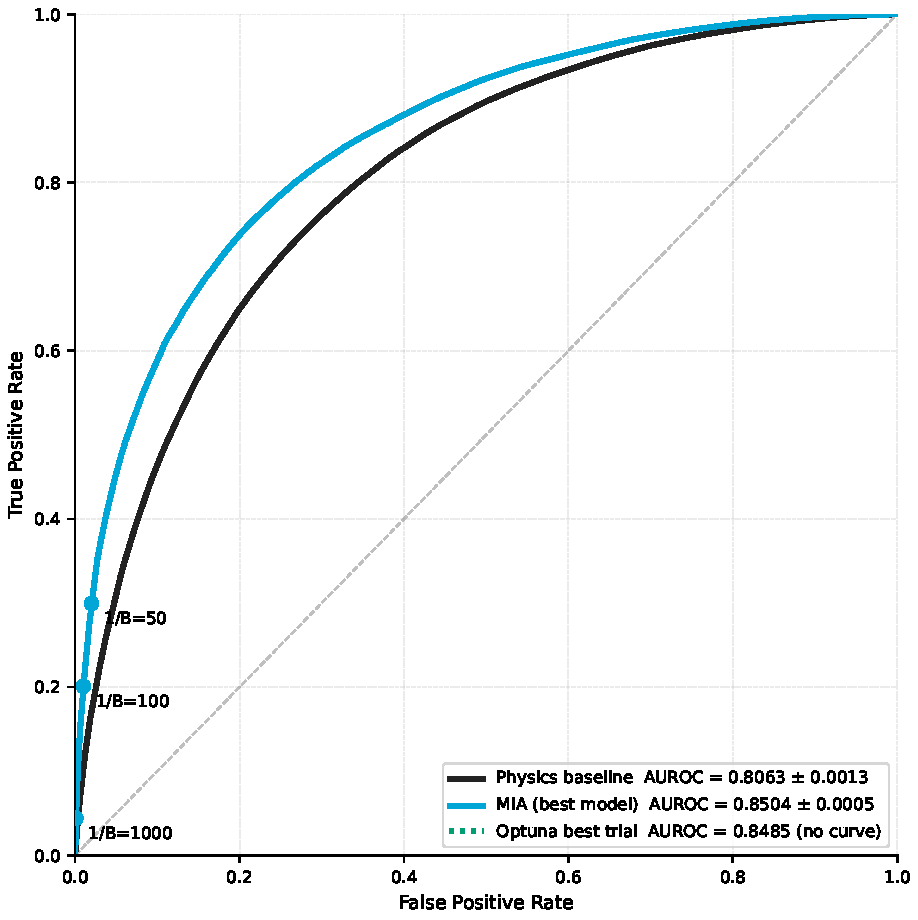
\includegraphics[width=0.85\textwidth]{figures/ch9/ch9_mia_roc_comparison.pdf}
  \caption{ROC curves for MIA (solid line, shaded band: $\pm$1\,std across five seeds)
    and the physics baseline (dashed, nine seeds). The Optuna best-trial AUROC
    (\num{0.8485}) is annotated in the legend as a scalar reference.
    Vertical dotted lines indicate the working points $1/B = 50$, $100$, and $1000$.
    Task: 4t vs.\ ttH+ttW+ttWW+ttZ.}
  \label{fig:ch9_roc}
\end{figure}

% ─────────────────────────────────────────────────────────────────────────────
\section{Discriminant Performance at Physics Working Points}
\label{sec:ch9_discriminant}

The AUROC summarises performance over all operating thresholds, but a hadron-collider
analysis selects a fixed working point determined by the tolerable background
contamination. Three background-rejection levels are considered here:
$1/B = 50$ (loose selection), $1/B = 100$ (standard), and $1/B = 1000$
(tight, high-purity). \Cref{tab:ch9_wp_comparison} lists the signal efficiency
$\varepsilon_{\mathrm{S}}$ achieved by each model at these working points.

\begin{table}[h]
\centering\small
\begin{tabular}{lrrr}
\toprule
Model & $\varepsilon_{\mathrm{S}}$ at $1/B=50$ & $\varepsilon_{\mathrm{S}}$ at $1/B=100$ & $\varepsilon_{\mathrm{S}}$ at $1/B=1000$ \\
\midrule
MIA (mean\,$\pm$\,std) & $\num{0.2987} \pm \num{0.0053}$ & $\num{0.1998} \pm \num{0.0046}$ & $\num{0.0458} \pm \num{0.0052}$ \\
Physics baseline       & $\num{0.1721} \pm \num{0.003}$  & $\num{0.1037} \pm \num{0.002}$  & $\num{0.0163} \pm \num{0.003}$  \\
\midrule
Ratio (MIA / baseline) & $\approx 1.74$ & $\approx 1.93$ & $\approx 2.81$ \\
\bottomrule
\end{tabular}
\caption{Signal efficiency $\varepsilon_{\mathrm{S}}$ at three background-rejection
  working points for MIA and the physics baseline.
  The ratio row shows the factor of improvement in signal yield at fixed background
  contamination. MIA uncertainties are one standard deviation across five seeds;
  baseline uncertainties are one standard deviation across nine seeds.}
\label{tab:ch9_wp_comparison}
\end{table}

The gain is modest at the loose working point: MIA retains approximately
$\varepsilon_{\mathrm{S}} = \num{0.299}$ of signal events against $\num{0.172}$
for the baseline, a factor of $\approx 1.74$. At $1/B = 100$ the improvement is
close to a factor of two ($\num{0.200}$ versus $\num{0.104}$), meaning that MIA
approximately doubles the signal yield for the same background contamination.
At the tight working point $1/B = 1000$ the gain grows to a factor of
$\approx 2.81$ ($\num{0.046}$ versus $\num{0.016}$), though the absolute signal
efficiencies at this threshold are small and the relative seed uncertainty is
correspondingly larger.

\Cref{fig:ch9_sig_eff_vs_bkg_rej} presents the signal efficiency as a function of
background rejection on a logarithmic scale, with the individual working-point values
labelled. The widening gap towards high background rejection indicates that MIA's
discriminant separates the tails of the score distributions more effectively than the
baseline, which is the regime most relevant to high-significance searches.

\begin{figure}[h]
  \centering
  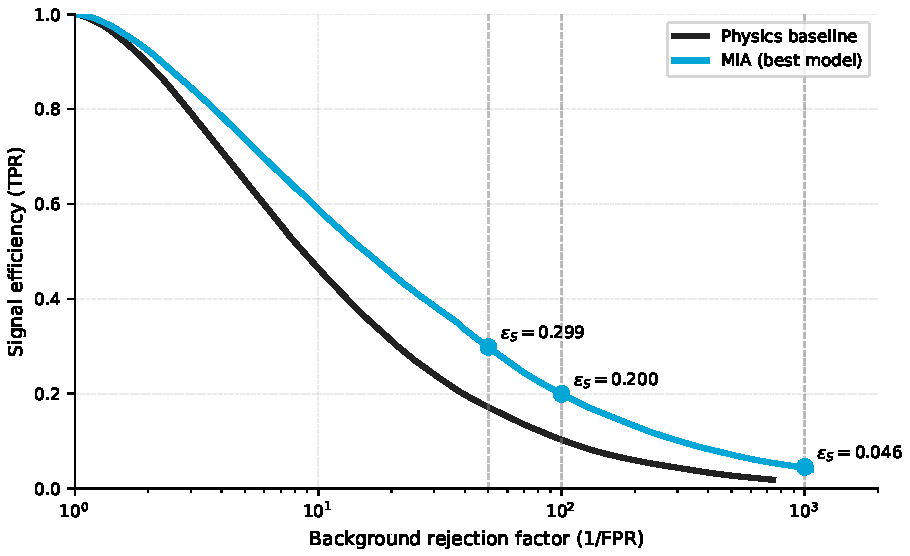
\includegraphics[width=0.85\textwidth]{figures/ch9/ch9_mia_sig_eff_vs_bkg_rej.pdf}
  \caption{Signal efficiency (TPR) as a function of background rejection ($1/\mathrm{FPR}$,
    logarithmic axis) for MIA (solid, shaded band) and the physics baseline (dashed).
    Labelled points indicate the three working points $1/B = 50$, $100$, and $1000$.
    The gap between the two curves widens towards high background rejection.}
  \label{fig:ch9_sig_eff_vs_bkg_rej}
\end{figure}

\Cref{fig:ch9_score_dist} shows the normalised discriminant score distributions for
signal and background events for both models. MIA produces a more pronounced
separation between the two distributions: the signal peak is shifted further towards
high scores and the background is more concentrated at low scores compared to the
physics baseline. The visual separation is consistent with the working-point gains
reported above.

\begin{figure}[h]
  \centering
  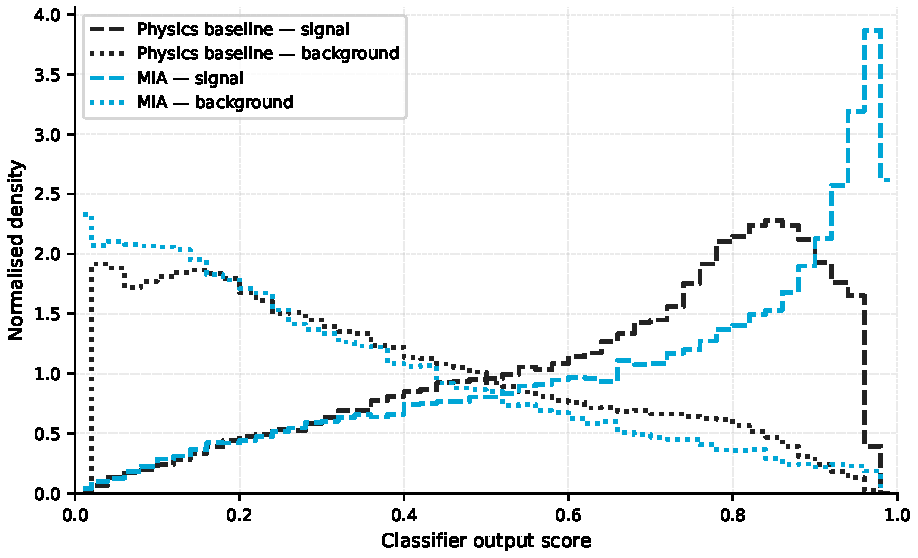
\includegraphics[width=0.85\textwidth]{figures/ch9/ch9_mia_score_distributions.pdf}
  \caption{Normalised discriminant score distributions for signal (4t) and background
    (ttH+ttW+ttWW+ttZ) events, comparing MIA (top) and the physics baseline (bottom).
    A clearer separation between the two distributions is visible for MIA.}
  \label{fig:ch9_score_dist}
\end{figure}

% ─────────────────────────────────────────────────────────────────────────────
\section{Illustrative Physics Reach}
\label{sec:ch9_physics_reach}

The signal efficiency improvements quantified in \cref{sec:ch9_discriminant} have a
direct physical interpretation: at fixed luminosity and background rate, retaining
more signal events increases the expected discovery significance. This section
provides an illustrative estimate of that gain using simplified assumptions. All
numbers are intended to demonstrate relative improvement between classifiers; they
are not predictions of the actual experimental sensitivity.

\subsection{Significance Estimator}
\label{subsec:ch9_significance_formula}

The expected significance of an excess is estimated via the formula

\begin{equation}
  Z = \frac{S}{\sqrt{B + (\delta_{\mathrm{syst}}\, B)^2}},
  \label{eq:ch9_significance}
\end{equation}

where $S$ and $B$ are the expected signal and background yields at the chosen score
threshold, and $\delta_{\mathrm{syst}} = 0.10$ is a flat, uncorrelated fractional
systematic uncertainty on the background. The systematic term $(\delta_{\mathrm{syst}}\,B)^2$
dominates over the statistical term $B$ when $B > 1/\delta_{\mathrm{syst}}^2 = 100$
events, which is the expected regime at HL-LHC luminosities for a broad score cut.
\Cref{eq:ch9_significance} is not a profile-likelihood ratio; it does not account for
nuisance parameters, signal systematics, or multiple signal regions. The plot in
\cref{fig:ch9_significance} is explicitly annotated "Not a full profile-likelihood fit."

\subsection{Assumptions}
\label{subsec:ch9_assumptions}

The calculation uses the following inputs, all stated on the figure:

\begin{itemize}
  \item $\sigma(4t) = \SI{12.0}{\femto\barn}$ — ATLAS measurement of the four-top
        cross-section~\cite{collaborationObservationFourtopquarkProduction2023};
  \item $\sigma(\mathrm{bkg}) = \SI{800}{\femto\barn}$ — order-of-magnitude
        placeholder for the combined ttH+ttW+ttWW+ttZ background, explicitly
        identified as approximate;
  \item $\mathcal{L} = \SI{300}{\per\femto\barn}$ — HL-LHC benchmark luminosity;
  \item $\delta_{\mathrm{syst}} = 10\%$ — flat systematic on background yield, uncorrelated.
\end{itemize}

Signal and background yields as a function of score threshold are computed from the
normalised test-set score distributions, scaled to the cross-sections and luminosity
above. The resulting $Z$ versus threshold curve therefore reflects the shape of the
classifier output, not an absolute prediction.

\subsection{Results}
\label{subsec:ch9_significance_results}

\Cref{fig:ch9_significance} shows $Z$ as a function of the score cut for MIA and the
physics baseline, together with reference lines at $Z = 2$ and $Z = 5$.

\begin{figure}[h]
  \centering
  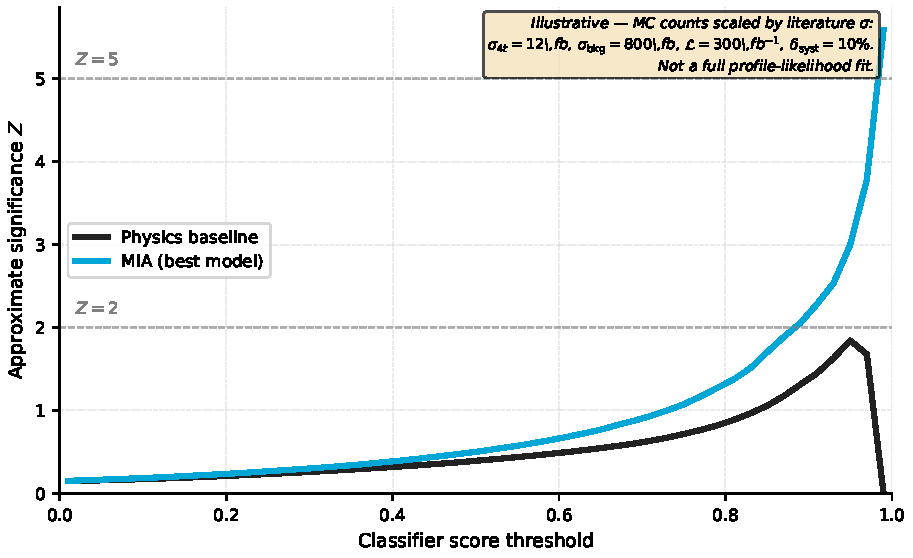
\includegraphics[width=0.85\textwidth]{figures/ch9/ch9_mia_significance_vs_threshold.pdf}
  \caption{Illustrative expected significance $Z$ as a function of score threshold for
    MIA (solid) and the physics baseline (dashed), computed using
    \cref{eq:ch9_significance} with $\sigma(4t) = \SI{12}{\femto\barn}$,
    $\sigma(\mathrm{bkg}) = \SI{800}{\femto\barn}$ (approximate placeholder),
    $\mathcal{L} = \SI{300}{\per\femto\barn}$, and a \SI{10}{\percent} flat background
    systematic. Horizontal dotted lines mark $Z = 2$ and $Z = 5$. The annotation
    "Not a full profile-likelihood fit" appears on the figure. These results are
    illustrative only.}
  \label{fig:ch9_significance}
\end{figure}

MIA reaches $Z = 2$ at a substantially looser score cut than the physics baseline.
This means that the MIA classifier extends the useful operating range of the
discriminant: analysis regions that would be background-dominated under the baseline
selection become accessible with MIA at the same significance level. In physical
terms, the factor-of-two improvement in signal efficiency at $1/B = 100$ translates
directly into a larger signal yield at fixed background rate, shifting the significance
curve upward and to the right.

The quantitative improvement at $Z = 5$ cannot be read reliably from this simplified
estimate because the systematic term dominates at high yields and the precise value
depends strongly on the background cross-section placeholder. The relative comparison
between MIA and the baseline is robust to this uncertainty because both curves use
the same background model.

% ─────────────────────────────────────────────────────────────────────────────
\section{Chapter Summary}
\label{sec:ch9_summary}

The MIA model, which accumulates all architectural recommendations from Chapters~5–8,
achieves a mean test AUROC of $\num{0.8504} \pm \num{0.0005}$ across five independent
seeds, compared with $\num{0.8063} \pm \num{0.0013}$ for the physics baseline
($\Delta\,\mathrm{AUROC} \approx \num{0.044}$). The gain is largest at high
background-rejection working points: at $1/B = 100$, MIA retains approximately twice
the signal yield of the baseline at the same background contamination ($\varepsilon_{\mathrm{S}}
= \num{0.200}$ versus $\num{0.104}$). An illustrative significance estimate under
HL-LHC conditions (\SI{300}{\per\femto\barn}, \SI{12}{\femto\barn} four-top cross-section,
\SI{10}{\percent} background systematic) shows that MIA reaches evidence-level
significance ($Z = 2$) at a substantially looser score cut than the baseline,
extending the effective operating range of the discriminant.

These results demonstrate that the sequence of architectural improvements motivated by
particle-physics considerations — differential attention, Lorentz-scalar biases, and
the scale identified by the Pareto analysis — translates into tangible improvements in
the physics reach of the classifier. A production physics analysis would require
additional steps: a profile-likelihood fit incorporating all signal regions and
systematic uncertainties, proper background modelling with data-driven components,
and a dedicated optimisation of the signal region boundaries. The present work
provides the architectural foundation and demonstrates that the physics sensitivity
scales with classifier quality in the expected direction.
